
\section{The Teacher Assistance Tools}
\label{sec:teach-assist-tools}

As discussed in the previous sections, MiGen's Teacher Assistance (TA)
Tools aim to support the teacher in monitoring students' progress on
tasks set for them to undertake in eXpresser, so that the teacher can
intervene with additional support for the class as a whole or for
individual students as she deems appropriate. 
% , e.g. in providing additional
% guidance, encouraging reflection, or setting new goals. 
% Of course,teachers are very well able to judge what constitutes progress and to
% support their students by appropriate prompts and nudges. As we
% discussed in Section 1, the problem for them is to do that effectively
% with a whole class of students as students are working on exploratory
% learning tasks using eXpresser all at the same time. MiGen's TA tools
% aim to support teachers by reducing their cognitive load and
% increasing their awareness of the classroom `state’.
%
The most detailed tool, and the one developed first chronologically, is the ST tool. 
So we begin with a description of that below, followed by the CD tool and the GA tool.

\subsection{Student Tracking}
\label{sec:student-tracking}

The ST tool monitors the occurrence of TI and TD indicators
generated by each student as they interact with the eXpresser. These
indicators are displayed in chronological order in a top-down timeline for each
student (see Figure~\ref{fig:STtool}), with one column for each student in the
class. Indicators whose occurrence indicates that the actions of the student
are consistent with what would be expected from productive interaction with respect
to the task at hand are coloured Green; indicators whose occurrence is regarded as 
an obstruction to productive interaction are coloured Red; indicators whose 
occurrence indicates that some aspect of the student's interaction may be positive 
or negative depending on context are coloured Yellow; and indicators relating
to feedback given by the system to the student are coloured Blue. 

Timelines can be made thinner or wider using a slider. Using
narrower timelines provides a general overview of all the students' 
timelines but does not show the text associated with the
indicators. Using wider timelines allows a more detailed exploration
of the indicators for a particular student. Timelines can also be made
shorter or longer (so that a vertical pixel represents a longer
or shorter time period). A shorter view allows the teacher to
undertake a general appraisal of all the students' actions so far. A
longer view allows the teacher to look in detail at students' interactions
during a specific time period.
Hovering with the cursor over one of the indicators 
provides further information: full name
of the indicator and precise time it occurred. For some indicators
additional information is also shown, e.g. for the indicator relating
to the accomplishment of a task goal, the full name of the goal. 

Indicators are displayed as horizontal bars or vertical lines
depending on whether they are event indicators or state
indicators. Event indicators relate to an action that happens at a
single time point, e.g. goal accomplished, pattern created, feedback
received. State indicators represent an aspect of the students'
interaction that is always monitored and has a value of `yes', `no' or
`maybe', e.g. `student is active', `student is animating
their model', `a plausible building block is in use'. 
%
The identification of the full set of indicators was achieved through
an iterative process undertaken as a joint activity with our teacher
collaborators during Phases A and B of the project. This resulted in the 
development of computational techniques to track over 50 different indicators. 
%
We refer the reader to~\cite{IEEE-TLT-TA} for a detailed description 
of the different categories of event and state indicators. 

However, during the classroom trials in Phase B it became evident that
it was infeasible for teachers to comprehend all of this information
at one time within the ST tool. Larger combinations of the indicators
would be useful for after-class analysis, but the number of indicators
to be displayed during the classroom session needed to be reduced.

The ST tool was therefore extended to allow the teacher to select
which indicators should be shown and which hidden, depending on the teacher's
current needs. For convenience, the indicators are divided into a
number of `families' which the teacher can select to be collectively
shown or hidden (the teacher can also select individual indicators to
be shown/hidden). The families of indicators are: event indicators,
state indicators, building-block related indicators, rule-related
indicators, and important indicators. This last category of `important'
indicators was identified by a team of pedagogical
experts in Phase C of the project (see Section 5 below) 
as being the most relevant for use by the teacher during the lesson. 
The default display of the current ST tool is with this family
of important indicators being shown; teachers can 
choose to `switch on' more indicators or `switch off' any of this
default set by means of the indicator-selection feature. 
The important indicators are all event indicators and
are the following:

\begin{itemize}
        	\item Number unlocked (i.e. variable created), displayed in Green;
        	
		\item Correct/incorrect local rule created (i.e. correct/incorrect allocation 
              of colour in a pattern), displayed in Green/Red;
        	
        	\item Correct/incorrect global rule created (i.e. correct/incorrect allocation
              of colour in the whole model), displayed in Green/Red;

    	    	\item Plausible/implausible building-block created (i.e. probably leads/does not lead
              to a correct solution for the task), Green/Red;
        	
        	\item Pattern made using a plausible/implausible building-block, Green/Red; 
        	
             
        	\item General solution created and animated; displayed in Green if
              the solution animates correctly, otherwise in Red;

        	\item Goal checked by system (i.e. one of the task goals
              has been detected as being accomplished by the system), Green;

        	\item Help requested by the student, Blue; 

        	\item Feedback shown to the student, Blue.

  \end{itemize}
 
Figure~\ref{fig:STtool} illustrates the ST tool visualisation, with the important
indicators and the `Tile placed' indicator selected. 
Looking at the left-most column, we see that student Anne Smith (all students'
names are aliases) has placed a tile, but has then been
detected as being inactive by the system. The system has displayed an appropriate
prompt to the student at this point, and she has resumed placing tiles. 
The system has detected `rhythm' from these tile placements ---
in the sense that the tiles placed on the canvas match part of the target model to
be constructed --- and has suggested that she create a building block from her tiles, 
which she has subsequently done. The system detects that this is a plausible
building block for the task at hand 
(shown by the occurrence of the green `Building Block created' indicator).
Anne continues to create a pattern from her building block, and to accomplish
the first goal of the task. 


\begin{figure}[htbp]
  \centering
  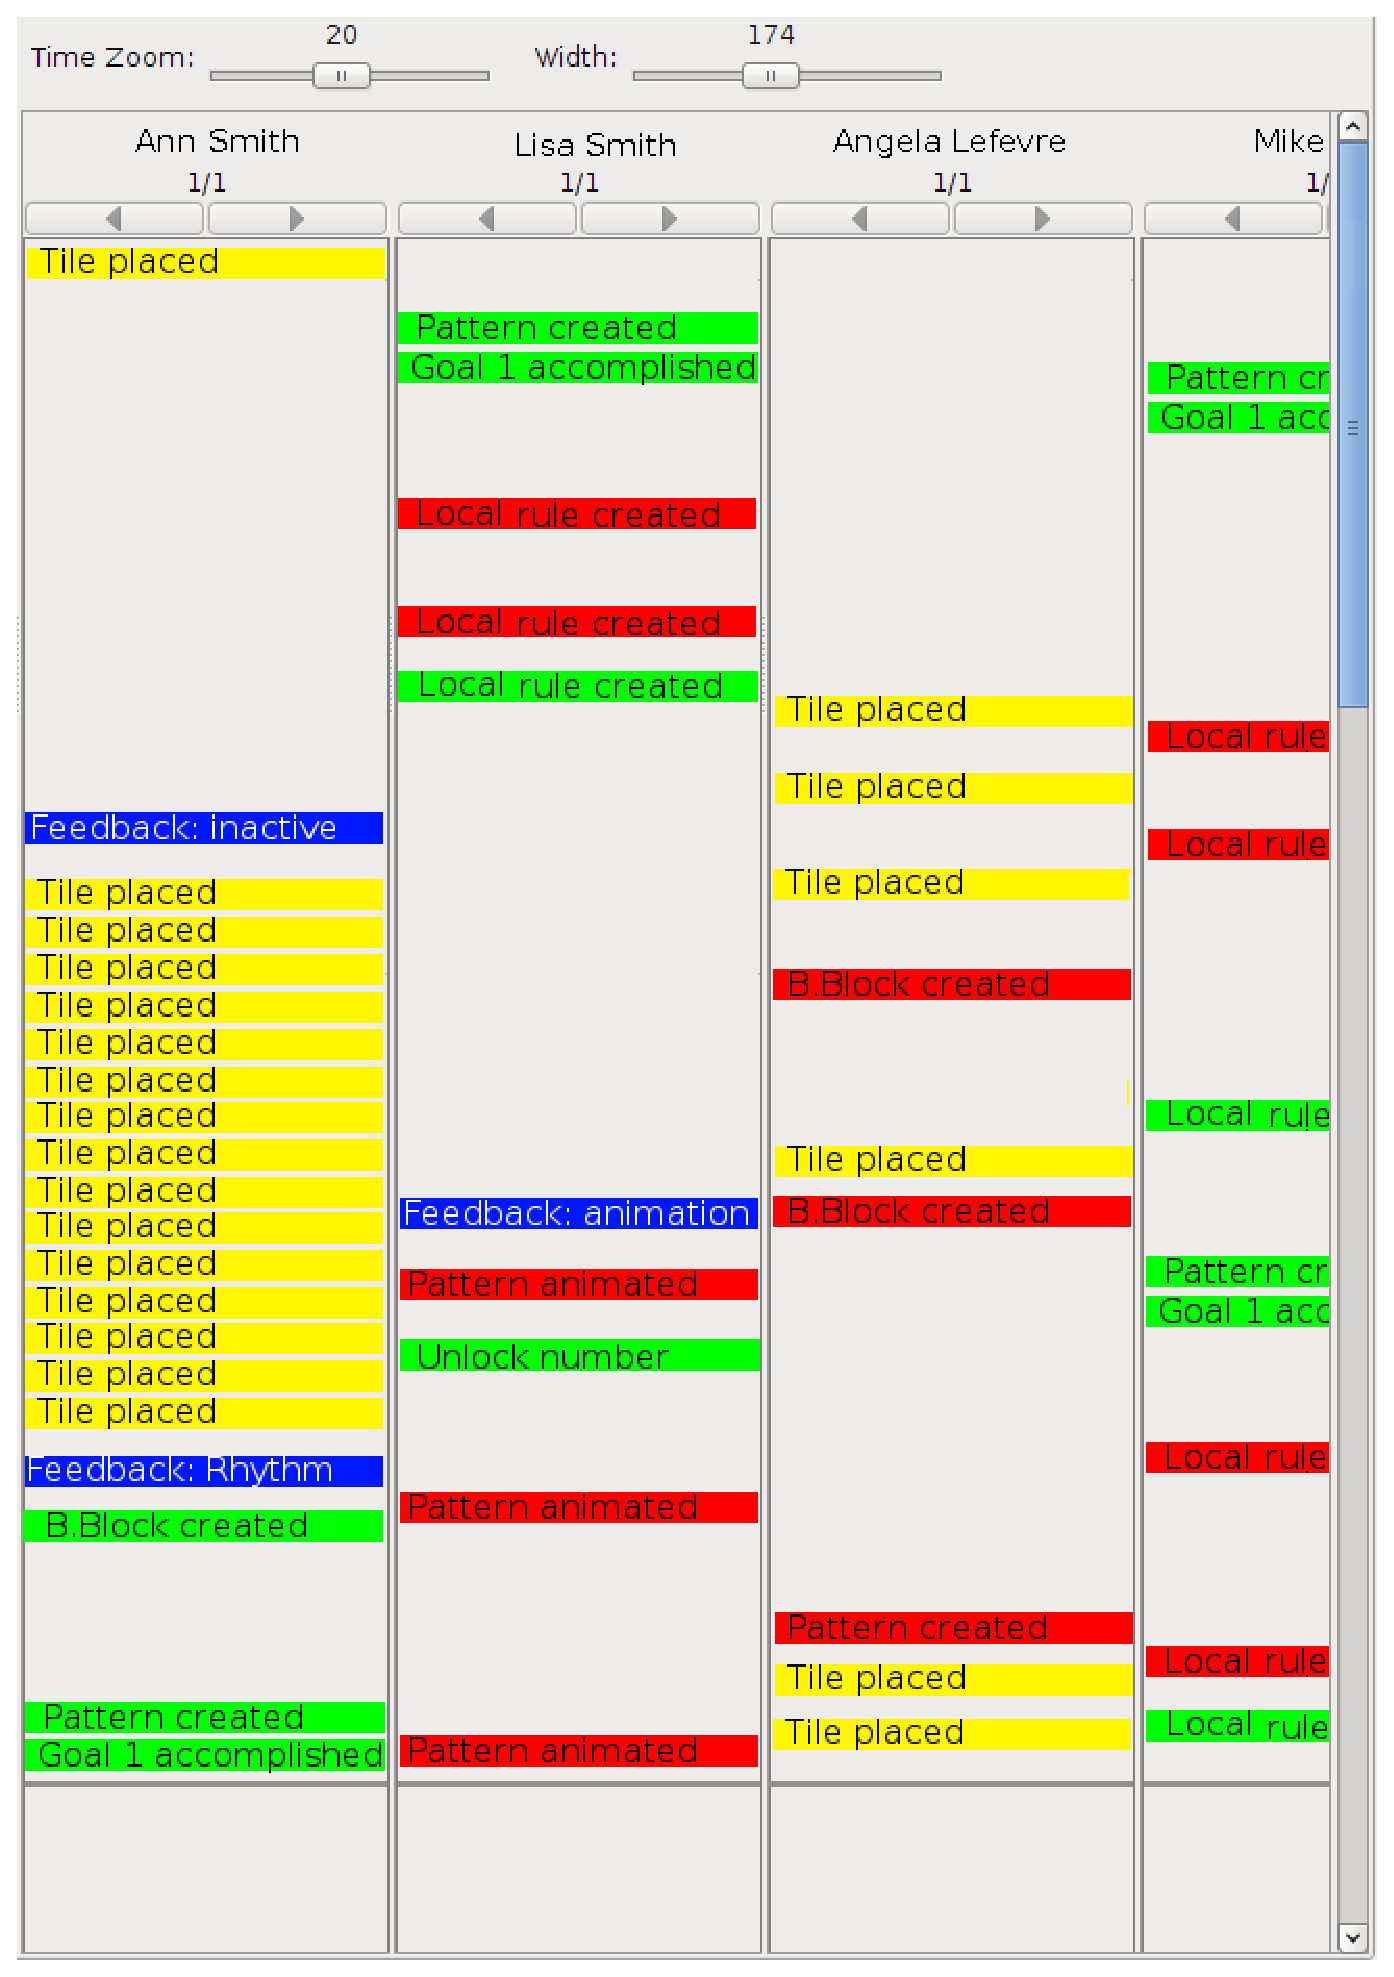
\includegraphics[width=\textwidth]{gfx/ta-st}
  \caption{Student Tracking visualisation. The first column shows how
    Ann Smith had little interest in the task at first, but make
    progress later thanks to support and feedback from the system.} 
  \label{fig:STtool}
\end{figure}

\subsection{Classroom Dynamics}
\label{sec:classroom-dynamics}

The CD tool gives the teacher an at-a-glance overview of which
students are currently engaged with the task and who may be in
difficulty and in need of the teacher's help (see Figure~\ref{fig:CDtool}, left-hand side). 
It represents each student in the classroom by a coloured circle, 
with the student's initials within it.  
Hovering over a circle with the cursor displays the student's full name. 
Clicking on a circle shows the student's 
current construction and current rule (see Figure~\ref{fig:CDtool}, right-hand side). 
The colour of a student's circle reflects the
student's current activity status as perceived by the system:
students shown in Green are working productively on
the task set as far as the system can tell; 
students shown in Amber have not interacted with the eXpresser for some time 
(by default, five minutes); 
%  Unless this is expected by the teacher (for example,
%  sometimes teachers interrupt the lesson to address the class and
%  explain some common misunderstanding), this usually means that the
%  student is distracted, for example talking to fellow student, or
%  playing games in their web-browser.
students shown in Red have requested help from the system
in a situation where the intelligent support cannot help
any further: at such times the eXpresser displays the
message ``The teacher will come to help you now'' 
and the student's circle becomes coloured Red in the CD tool 
in order to attract the attention of the teacher.

\begin{figure}[hbtp]
  \centering
  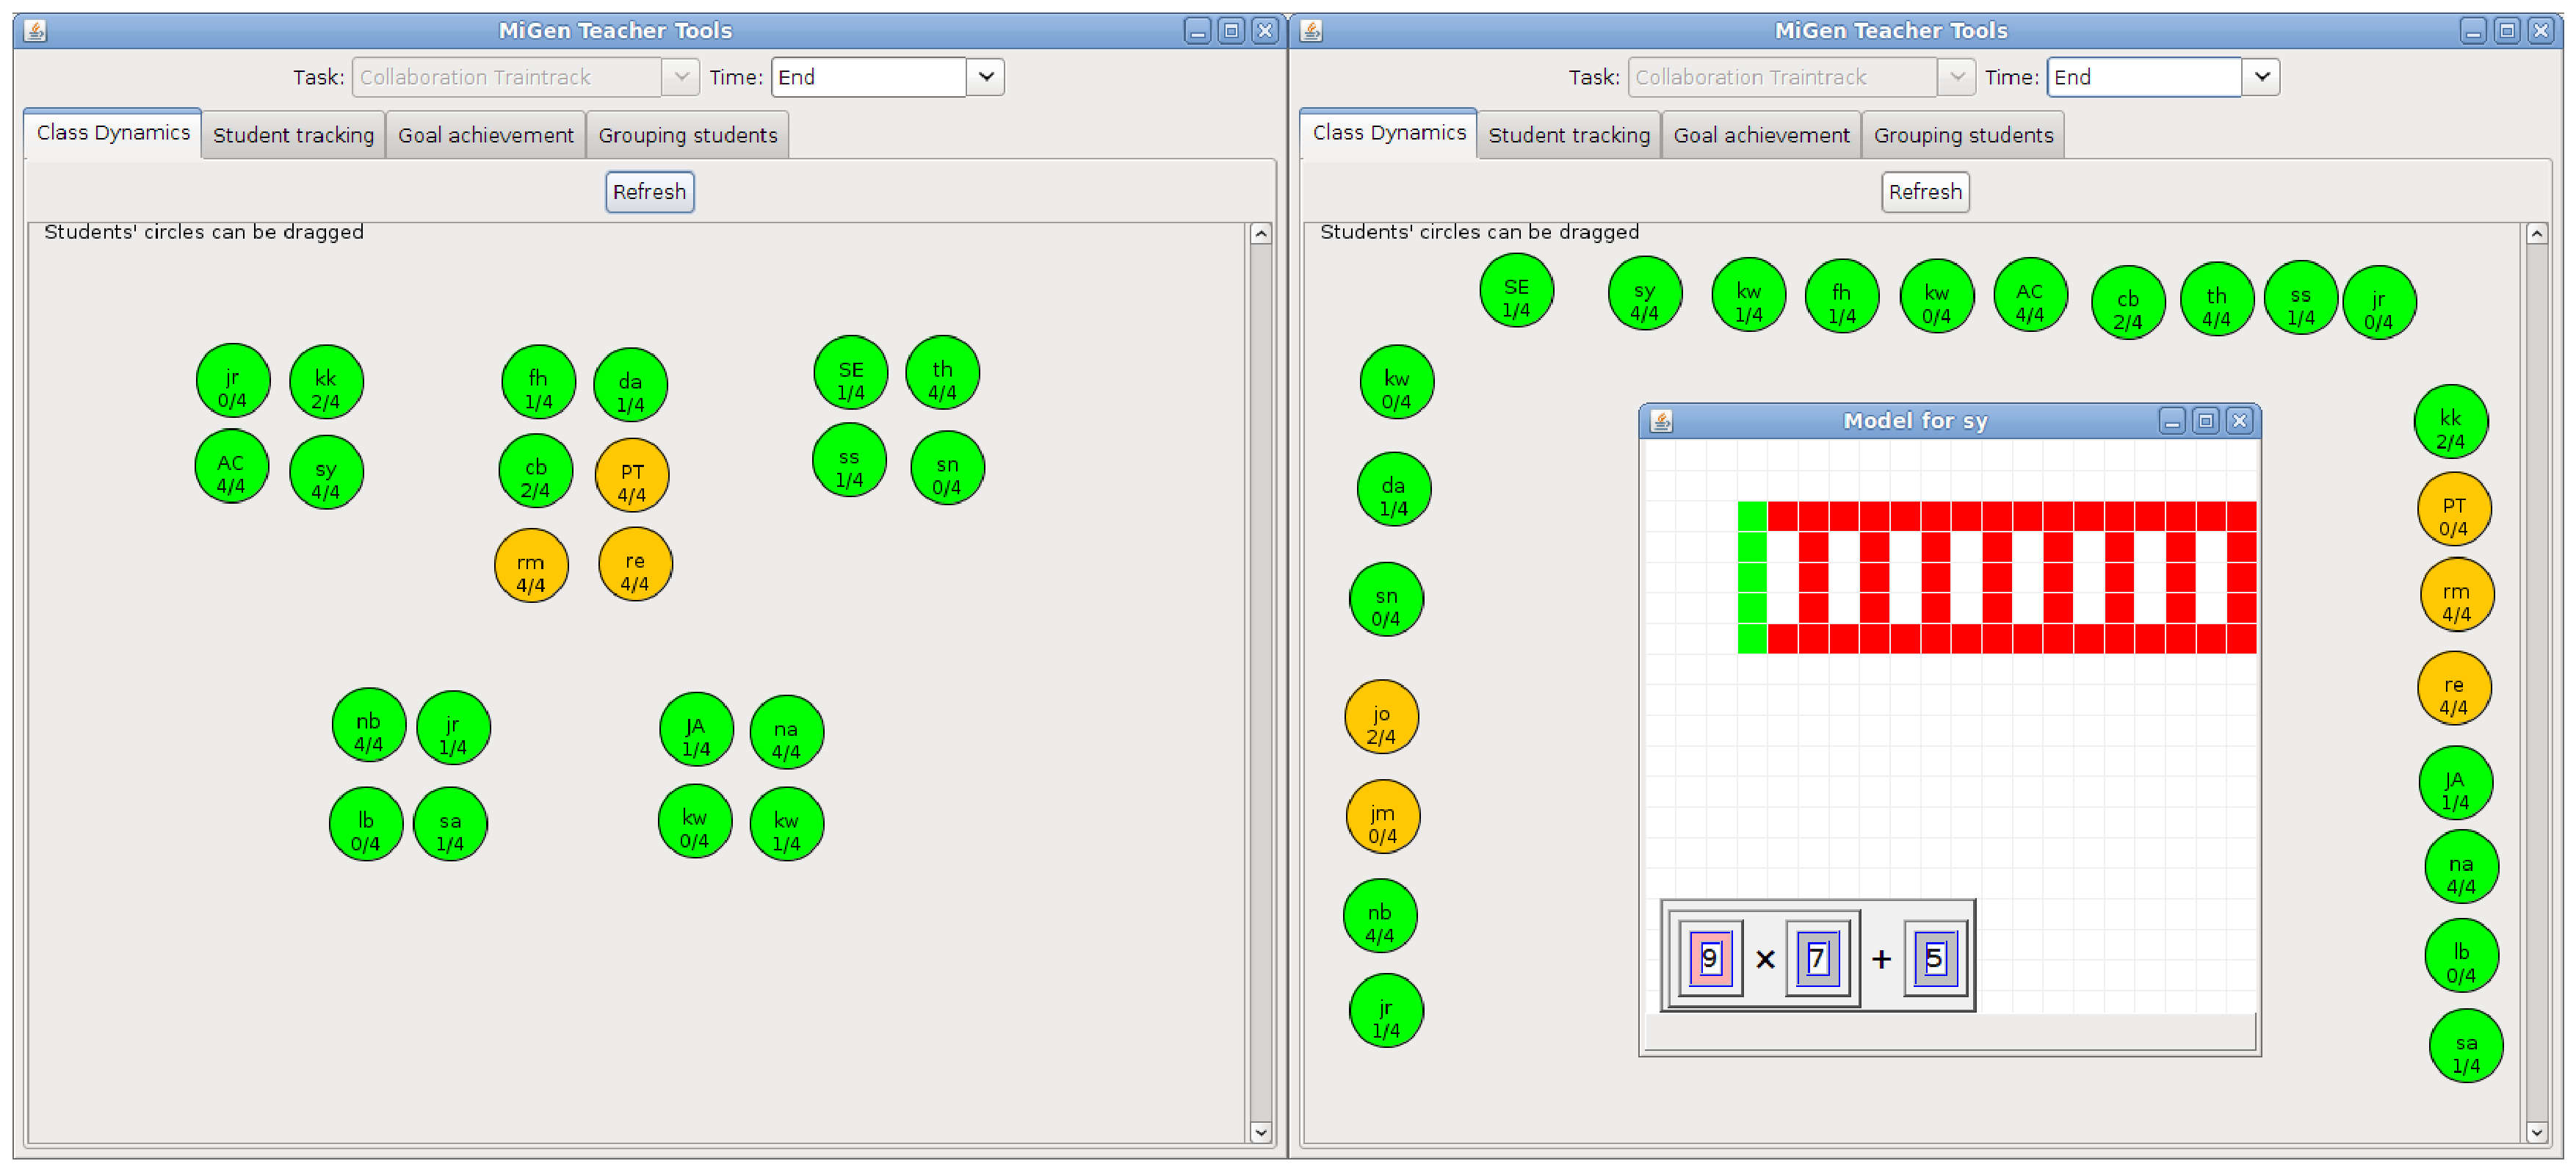
\includegraphics[width=\textwidth]{gfx/ta-cd}
  \caption{Class Dynamics tool. On the left, a classroom with the
    students sitting on tables. On the right, another classroom with
    students sitting in desks around the wall; in this case, the
    teacher has clicked on one of the students to see their
    construction and rule. }
  \label{fig:CDtool}
\end{figure}

The circles representing the students can be dragged and moved around on
the canvas. This enables teachers to set up the display so that the
position of the circles matches the students'
spatial positioning in the classroom. This helps the teacher to match
the information displayed in the CD tool with her own observations. 
It also helps the teacher to identify situations that
may be location-dependent. For example, if several students seated at
the same table show as Amber this may indicate that they are
distracting each other and that the teacher should intervene to
refocus their attention on the task.

An optional feature in the CD tool shows within each student's circle the number of
goals achieved so far, as a fraction of the total number of goals of the task. 
For example, if a student has achieved
two of the goals of a task that has four goals, this would show 
as 2/4. This does not provide information about {\em which} of the task goals have
been achieved and generally task goals can be achieved in different
orders. More detailed information about the achievement of task goals
is shown by the Goal Achievement tool. 

\subsection{Goal Achievement}
\label{sec:goal-achievement}

%The Goal Achievement tool shows detailed information about the
%achievement of task goals by students. It allows the teacher to decide
%if more explanation is needed for the class as a whole relating to any
%of the task goals, if a student who has finished the task can be asked
%to help one of the other students, or if the class is ready to move on
%to the next task. 

\begin{figure}[hbtp]
  \centering
  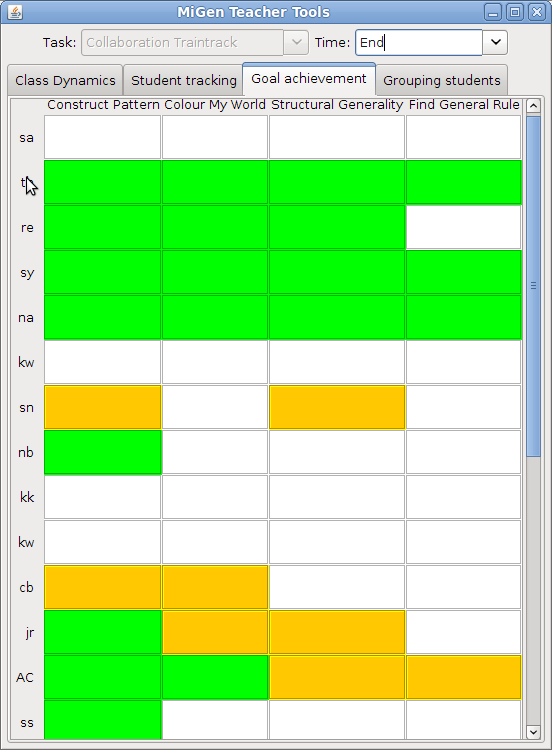
\includegraphics[width=8cm]{gfx/ta-ga}
  \caption{Goal Achievement tool. It can be seen that some students
    have achieved all or most tasks, some students are not making any
    progress, and some students are moving back and forth.}
  \label{fig:GAtool}
\end{figure}

The GA tool shows a tabular display of students and task goals (see Figure~\ref{fig:GAtool}).
Each row of the table shows the progress of one student (identified by
their initials) in completing the task goals. Each column 
shows the completion status of one task goal for all students. The
names of the tasks are shown at the top and the bottom of the
columns. Each student has several cells next to their name, one
cell for each task goal. Hovering over a cell with the cursor
displays a full description of the goal, the name of
the student and the achievement status of that goal for that
student. We note that the goal achievement information displayed by the GA
tool is inferred by the eGeneraliser and may not necessarily
correspond to the information about goal achievement provided
by the students themselves in their Activity Document: sometimes
students tick as `done' task goals they believe they have achieved
but which the system infers as not actually being achieved;
conversely, sometimes students do not tick as `done' task goals
(e.g.~they forget) that
the system infers as being achieved.
 
The GA tool uses colour coding to identify the current
status of a task goal for each student:
a White cell shows that a goal has not been achieved yet;
a Green cell shows that the goal is currently being achieved 
by the student's construction; 
an Amber cell shows that the goal has been achieved
by the student during the course of the current task, but is not being
achieved by the student's current construction.
A task goal can appear as Amber for several reasons. For example, some
students may finish the task earlier than others and the system
gives such students the opportunity to undertake the task again but
this time following a different construction approach; such students
would appear with all their task goal cells coloured Amber in the GA
tool and with the cells gradually turning to Green again. 
Some students may not recognise that they have
accomplished a task goal and their further interaction with eXpresser
may result in a situation where the goal is no longer being achieved, 
either accidentally (e.g. a pattern was coloured generally but then a
variable is deleted) or in an explicit attempt to achieve some other
task goal (e.g. in order to relate two patterns via the same
variable, the student may temporarily leave them uncoloured). 
Using three colours for visualising the task goal
achievement information allows the teacher to differentiate between
those students who have moved back and forth taking different
construction approaches to the task and those students who are having
problems completing the task and cannot advance.


\subsection{Time-stop Functionality}
\label{sec:time-stop-func}

This is a cross-tool functionality provided by all the TA tools. It
allows the user to select a specific point in time, $t$, with respect to
which the ST, CD and GA visualisations are generated. The tools ignore
all indicator occurrences after that time point, allowing analysis of
the situation at that particular time. In particular, the ST tool
shows the history of indicator occurrences for all students up to time
$t$, the CD tool shows the classroom status at time $t$, and the
GA tool shows the goal achievement information at time $t$.  If the
time point selected is in the future, or if no time point is
explicitly selected, the tools show the current situation by default.
 
The time-stop functionality has several important uses. Firstly, it allows
teachers to see information relating to a point in time in the past
in order to better understand the context of a particular situation. 
For example, using the ST tool after the lesson, the
teacher may observe an unexpected sequence of
indicators for a student. The teacher can use the CD tool `frozen'�
at that particular moment to check what was the status of other
students nearby, e.g. were they all inactive/in need of help?
%
Secondly, the time-stop functionality allows the TA tools to be used by
the research team to visualise ---for research purposes--- the students' 
interaction data arising from each classroom session.
%
Thirdly, being able to use the interaction data gathered from classroom trials 
and to present that data via the TA tools `frozen'�at particular moments in 
time enables the evaluation of the TA tools with a far larger number of teachers than 
those who are able to participate in classroom trials, allowing
the research team to pose questions to evaluation participants 
as if they were in the real classroom at that precise moment. 
%
%Although the situation is not
%identical (the evaluation participants were not under pressure from
%students asking for their help or trying to keep the lesson on track
%while they used the TA tools), having access to a much larger number
%of teachers who could participate in the evaluation of the TA tools
%even if they could not trial the TA tools in their own classrooms was
%extremely helpful in the design and evaluation of the tools, as
%will be discussed below.

\subsection{Example of Use of the TA tools}
\label{sec:example-use}

In order to facilitate readers' understanding of the TA tools, we now 
briefly describe how they may be used in a typical classroom session. 
At the start of the session, the teacher introduces the lesson 
and instructs students to open the eXpresser on their computers and to read
about the current task within the Activity Document. While they 
are doing this, she opens up the TA tools on her computer, typically a tablet. 
For the first few minutes of the lesson, the teacher walks around the classroom 
to make sure that students are focussing on the task at hand and that they
understand the task goals. Once students have begun working on the
task in eXpresser, the teacher can take a step back and use the TA tools to 
monitor students' progress. 

Most of the time, the teacher will have the CD tool selected for display. 
If any students show as Amber, she approaches them and encourages them to
resume working on the task. 
%
% The CD tool allows
% the teacher to detect that students that are engaged with the
% computer are not engaged with the learning task at hand: maybe they
% are wasting time on a social network or playing a web game. She does
% not need to see every screen to check student engagement: the CD tools
% does the job.
%
Some students may call out to the teacher for help, or may raise their hands.
The teacher encourages them to first seek help from the system:
``If the system cannot help you, then I will come to you'' she tells them,
knowing that students in such a situation will automatically appear 
red in the CD tool. 
If a student does appear red, the teacher 
goes to the student to help, since she knows that this is a situation where
the system's intelligent support cannot help the student any further. 
If more than one student appears red, she clicks on all those students' circles 
to see their current models and rules, so that she can prioritise helping 
the students who seem to be having the most difficulty. 

From time to time, the teacher looks also at the GA tool.
Knowing which students have accomplished all the task goals allows
the teacher to offer them additional activities.  
Other students may be advancing more slowly; the teacher can use this information to 
set them additional homework so that they can catch up with 
their peers if they need more time than is available in the lesson. 
If the GA tool shows that many students are not achieving a particular task goal, 
the teacher can interrupt the lesson to help all the students at the same
time by clarifying a goal that may be unclear or by providing additional
guidance to help students' understanding.

At the end of the lesson, the teacher can use the ST to examine in detail what 
specific students have done. For example, if the teacher explained during the lesson
to one student how to relate two patterns by using the same variable, 
she can check whether the student started doing this right away or 
required a period of `trial and error' to understand the concept.

%%% Local Variables:
%%% mode: latex
%%% TeX-master: "main"
%%% End:
